\documentclass{article}
\usepackage{lmodern}


% if you need to pass options to natbib, use, e.g.:
%     \PassOptionsToPackage{numbers, compress}{natbib}
% before loading neurips_2025
\usepackage{xcolor}
\usepackage{graphicx}
\usepackage{subcaption}
\usepackage{tikz}
\usepackage{array}

% Define a new color environment
\newenvironment{cyanpar}{\color{cyan}}{}

\usepackage{caption}
\usepackage{subcaption}
\usepackage{array}
\usepackage{multirow}
\input{maths.tex}% ready for submission
%\usepackage{neurips_2025}
\usepackage{graphicx} % Required for \resizebox
\usepackage{xspace}
\newcommand{\mmdit}{\textit{MM-DiT}\xspace}
% to compile a preprint version, e.g., for submission to aRxiv, add add the
% [preprint] option:
%     \usepackage[preprint]{neurips_2025}


% to compile a camera-ready version, add the [final] option, e.g.:
%     \usepackage[final]{neurips_2025}

%\PassOptionsToPackage{square,numbers}{natbib}

% to avoid loading the natbib package, add option nonatbib:
\usepackage[nonatbib]{neurips_2025}
\usepackage[square,numbers,sort]{natbib}

\usepackage[utf8]{inputenc} % allow utf-8 input
\usepackage[T1]{fontenc}    % use 8-bit T1 fonts
\usepackage{hyperref}       % hyperlinks
\usepackage{url}            % simple URL typesetting
\usepackage{booktabs}       % professional-quality tables
\usepackage{amsfonts}       % blackboard math symbols
\usepackage{nicefrac}       % compact symbols for 1/2, etc.
\usepackage{microtype}      % microtypography
\usepackage{xcolor}         % colors
\usepackage{amsmath}
\usepackage{wrapfig}
% \title{CannyEdit: Regional Image Editing with Canny Edge Guidance in Pretrained Diffusion Models}

% \title{CannyEdit: Regional Image Editing via Selective Canny Control in Pretrained Diffusion Models}

% \title{RTSC-Edit: Training-free Image Editing via \underline{R}egional \underline{T}ext Guidance and \underline{S}elective \underline{C}anny Control}

\usepackage{enumitem}

\usepackage[normalem]{ulem}
\newcommand{\kc}[1]{\textcolor{blue}{#1}}
\newcommand{\kcc}[1]{\textcolor{black}{#1}}

% \usepackage{lmodern}
% \usepackage[T1]{fontenc}

\title{CannyEdit: Selective Canny Control and Dual-Prompt Guidance for Training-free Image Editing}
% \title{CannyEdit: Seamless Image Editing via Selective Canny Control and Dual-Prompt Guidance}



% The \author macro works with any number of authors. There are two commands
% used to separate the names and addresses of multiple authors: \And and \AND.
%
% Using \And between authors leaves it to LaTeX to determine where to break the
% lines. Using \AND forces a line break at that point. So, if LaTeX puts 3 of 4
% authors names on the first line, and the last on the second line, try using
% \AND instead of \And before the third author name.


\author{%
  David S.~Hippocampus\thanks{Use footnote for providing further information
    about author (webpage, alternative address)---\emph{not} for acknowledging
    funding agencies.} \\
  Department of Computer Science\\
  Cranberry-Lemon University\\
  Pittsburgh, PA 15213 \\
  \texttt{hippo@cs.cranberry-lemon.edu} \\
  % examples of more authors
  % \And
  % Coauthor \\
  % Affiliation \\
  % Address \\
  % \texttt{email} \\
  % \AND
  % Coauthor \\
  % Affiliation \\
  % Address \\
  % \texttt{email} \\
  % \And
  % Coauthor \\
  % Affiliation \\
  % Address \\
  % \texttt{email} \\
  % \And
  % Coauthor \\
  % Affiliation \\
  % Address \\
  % \texttt{email} \\
}




\begin{document}

\maketitle


\begin{abstract}
Recent advances in text-to-image (T2I) models have enabled training-free regional image editing by leveraging the generative priors of foundation models. However, existing methods struggle to balance text adherence in edited regions, context fidelity in unedited areas, and seamless integration of edits. We introduce \textbf{\textit{CannyEdit}}, a novel training-free framework that addresses these challenges through two key innovations: (1) \textbf{\textit{Selective Canny Control}}, which masks the structural guidance of Canny ControlNet in user-specified editable regions while strictly preserving the source image’s details in unedited areas via inversion-phase ControlNet information retention. This enables precise, text-driven edits without compromising contextual integrity. (2) \textbf{\textit{Dual-Prompt Guidance}}, which combines local prompts for object-specific edits with a global target prompt to maintain coherent scene interactions. On real-world image editing tasks (addition, replacement, removal), CannyEdit outperforms prior methods like KV-Edit, achieving a 2.93\%–10.49\% improvement in the balance of text adherence and context fidelity. In terms of editing seamlessness, user studies reveal only 49.2\% of general users and 42.0\% of AIGC experts identified CannyEdit's results as AI-edited when paired with real images without edits, versus 76.08–89.09\% for competitor methods. The code and benchmark used in this paper will be made publicly available upon acceptance.
\end{abstract}
%demonstrating superior seamlessness. Our work establishes a flexible, training-free paradigm for high-fidelity regional editing, advancing the practical deployment of T2I models in real-world applications.


\begin{figure}[h!]
\centering
\begin{tabular}{@{\hskip 1pt} p{\dimexpr\textwidth/9\relax}
                   @{\hskip 1pt} p{\dimexpr\textwidth/9\relax}
                   @{\hskip 1pt} p{\dimexpr\textwidth/9\relax}
                   @{\hskip 1pt} p{\dimexpr\textwidth/9\relax}
                   @{\hskip 5pt} p{\dimexpr\textwidth/9\relax}
                   @{\hskip 1pt} p{\dimexpr\textwidth/9\relax}
                   @{\hskip 1pt} p{\dimexpr\textwidth/9\relax}
                   @{\hskip 1pt} p{\dimexpr\textwidth/9\relax} @{}}

\multicolumn{4}{c}{\tiny (a) \textbf{Add} a woman with her dog and a student reading book on the lawn.} & 
\multicolumn{4}{c}{\tiny (b) \textbf{Add} a person running on the street.}  \\
\includegraphics[width=\linewidth,  height=1.5cm]{figures/f1/1_1.png} &
\includegraphics[width=\linewidth,  height=1.5cm]{figures/f1/1_2.png} &
\includegraphics[width=\linewidth,  height=1.5cm]{figures/f1/1_3.png} &
\includegraphics[width=\linewidth,  height=1.5cm]{figures/f1/1_4.png} &
\includegraphics[width=\linewidth,  height=1.5cm]{figures/f1/4_1.png} &
\includegraphics[width=\linewidth,  height=1.5cm]{figures/f1/4_2.jpg} &
\includegraphics[width=\linewidth,  height=1.5cm]{figures/f1/4_3.jpg} &
\includegraphics[width=\linewidth,  height=1.5cm]{figures/f1/4_4.png} \\[-1pt]

\multicolumn{4}{c}{\tiny (c) \textbf{Replace} the woman tennis player with a man tennis player.} & 
\multicolumn{4}{c}{\tiny (d) \textbf{Add} a baseball catcher on the field.} \\
\includegraphics[width=\linewidth,  height=1.5cm]{figures/f1/2_1.jpg} &
\includegraphics[width=\linewidth,  height=1.5cm]{figures/f1/2_2.jpg} &
\includegraphics[width=\linewidth,  height=1.5cm]{figures/f1/2_3.jpg} &
\includegraphics[width=\linewidth,  height=1.5cm]{figures/f1/2_4.jpg} &
\includegraphics[width=\linewidth,  height=1.5cm]{figures/f1/5_1.jpeg} &
\includegraphics[width=\linewidth,  height=1.5cm]{figures/f1/5_2.jpeg} &
\includegraphics[width=\linewidth,  height=1.5cm]{figures/f1/5_3.jpeg} &
\includegraphics[width=\linewidth,  height=1.5cm]{figures/f1/5_4.png} \\[-1pt]

\multicolumn{4}{c}{\tiny (e) \textbf{Remove} the umbrellas.} &
\multicolumn{4}{c}{\tiny (f) \textbf{Replace} the pepper with three apples.} \\
\includegraphics[width=\linewidth,  height=1.5cm]{figures/f1/3_1.jpg} &
\includegraphics[width=\linewidth,  height=1.5cm]{figures/f1/3_2.jpg} &
\includegraphics[width=\linewidth,  height=1.5cm]{figures/f1/3_3.jpg} &
\includegraphics[width=\linewidth,  height=1.5cm]{figures/f1/3_4.png} &
\includegraphics[width=\linewidth,  height=1.5cm]{figures/f1/6_1.jpg} &
\includegraphics[width=\linewidth,  height=1.5cm]{figures/f1/6_2.png} &
\includegraphics[width=\linewidth,  height=1.5cm]{figures/f1/6_3.jpg} &
\includegraphics[width=\linewidth,  height=1.5cm]{figures/f1/6_4.png} \\
\multicolumn{1}{c}{{\scriptsize Input}} &\multicolumn{1}{c}{{\scriptsize CannyEdit}} &\multicolumn{1}{c}{{\scriptsize KV-Edit }}&\multicolumn{1}{c}{{\scriptsize GPT-4o }} &\multicolumn{1}{c}{{\scriptsize Input}} &\multicolumn{1}{c}{{\scriptsize CannyEdit}} &\multicolumn{1}{c}{{\scriptsize KV-Edit}}&\multicolumn{1}{c}{{\scriptsize GPT-4o }} \\
\end{tabular}
\caption{Examples of edits using our CannyEdit, KV-Edit~\citep{zhu2025kv}, and GPT-4o~\citep{OpenAI2025Introducing4O}. Actual text prompts and masks are omitted here. For more details, see Appendix~F.1.}
\label{logo}
\end{figure}

\section{Introduction}
\label{Sec:intro}
%

Recent advances in text-to-image (T2I) models have achieved substantial progress in quality and controllability \citep{rombach2022high,betker2023improving,chen2023pixart,esser2024scaling,blackforest2024FLUX}. These advancements have enabled diverse downstream applications, utilizing their enhanced quality, efficiency, and versatility. In this work, we address one of the most challenging applications: \emph{region-based image editing}, which entails modifying user-specified image areas (e.g., adding, replacing, or removing objects) while maintaining {overall image consistency}.
Region-based image editing extends standard T2I generation by introducing a critical constraint: the generated content must align not only with the text prompt {(\textbf{\textit{Text Adherence}})} but also with the existing visual context of the image {(\textbf{\textit{Context Fidelity}})}.
This problem is commonly known as the \textit{editability-fidelity trade-off}.



A straightforward approach to region-based image editing involves collecting paired training data (before and after editing), along with corresponding text prompts, to train models for editing \citep{brooks2023instructpix2pix, zhang2023magicbrush, wasserman2024paint, li2024brushedit, hui2024hq, wei2024omniedit}. However, these methods often struggle to generalize beyond their training distribution--particularly in cases requiring realistic interactions, such as inserting people into complex scenes. This limitation is largely due to the lack of diverse, high-quality training data capturing such interactions.


To overcome this limitation, another line of research taps into the emergent capability of foundation T2I models to capture realistic object interactions learned from large-scale datasets.{These training-free approaches, initially developed upon UNet-based diffusion models~\citep{hertz2022prompt, cao2023masactrl, tumanyan2023plug}, has gradually shifted to leveraging more advanced rectified-flow-based multi-modal diffusion transformers (MM-DiTs)~\citep{rout2024semantic, wang2024taming, deng2024fireflow, tewel2025addit, zhu2025kv}.
A key advantage of MM-DiTs is their flexibility to control the generation process, e.g., one can inject the query/key/value of source-image tokens (obtained via inversion \citep{deng2024fireflow,rout2024semantic,wang2024taming}) into that of the generated tokens at each denoising timestep, improving context fidelity.}
However, the improved context fidelity often comes at a cost of text adherence, as exemplified by results of RFSolver-Edit~\citep{wang2024taming} under different injection steps in  Figure \ref{fig2} (b.1-b.6), where it is unable to strike a good balance between the two criteria. A quantitative study on this is shown in Figure \ref{treadline}.






\begin{wrapfigure}{r}{0.4\textwidth}
  \vspace{-12pt} % Optional: to pull the figure up slightly
    \includegraphics[width=1\linewidth]{figures/tl4.png}
    \vspace{-6mm}
    \caption{Quantitative study shows that CannyEdit achieves the best editability-fidelity trade-off under varying hyperparameter settings. The technical details of the graph are in Appendix F.1.}
    \label{treadline}
      \vspace{-9pt} % Optional: reduce space below the figure
\end{wrapfigure}

To achieve a better trade-off, KV-Edit~\citep{zhu2025kv} introduces user-provided masks to separate regions to be edited from those to be preserved.
During generation, KV-Edit only updates the image tokens in the unmasked regions while keeping the masked regions intact.
Although this greatly improves the trade-off (as shown by the orange points in Figure~\ref{treadline}), KV-Edit sometimes produces conspicuous artifacts and inconsistencies at mask boundaries, especially when the mask is not precise.
Typical examples are shown in Figure~\ref{logo} (b, d) and Figure~\ref{fig2} (c.1, d.1).
% This creates a burden on the users, potentially impacting their experience.
This imperfection highlights another key aspect of region-based image editing: \textbf{\textit{Editing Seamlessness}}, which is essential to good user experience.
We hypothesize that the boundary artifacts of KV-Edit originate from its hard context replacement strategy, which ensures context fidelity but breaks the interdependency necessary for smooth boundary transitions.



Building upon these insights, we propose a novel training-free image editing method, \emph{CannyEdit}, that achieves the state of the art in editability-fidelity trade-off, in addition to a significant qualitative improvement in seamlessness as validated by a comprehensive user study.
Specifically, our approach involves two key innovations.
First, we utilize Canny ControlNet's outputs~\citep{zhang2023adding} in a selective way to relax the structural constraints in the desired edit region while preserving the original image layout elsewhere.
Second, we propose a dual-prompt strategy that uses a \emph{local prompt} to provide fine guidance to edit regions along with a global \emph{target prompt} to ensure coherence between the edit regions and the context.

\begin{figure}[t]

    \centering
    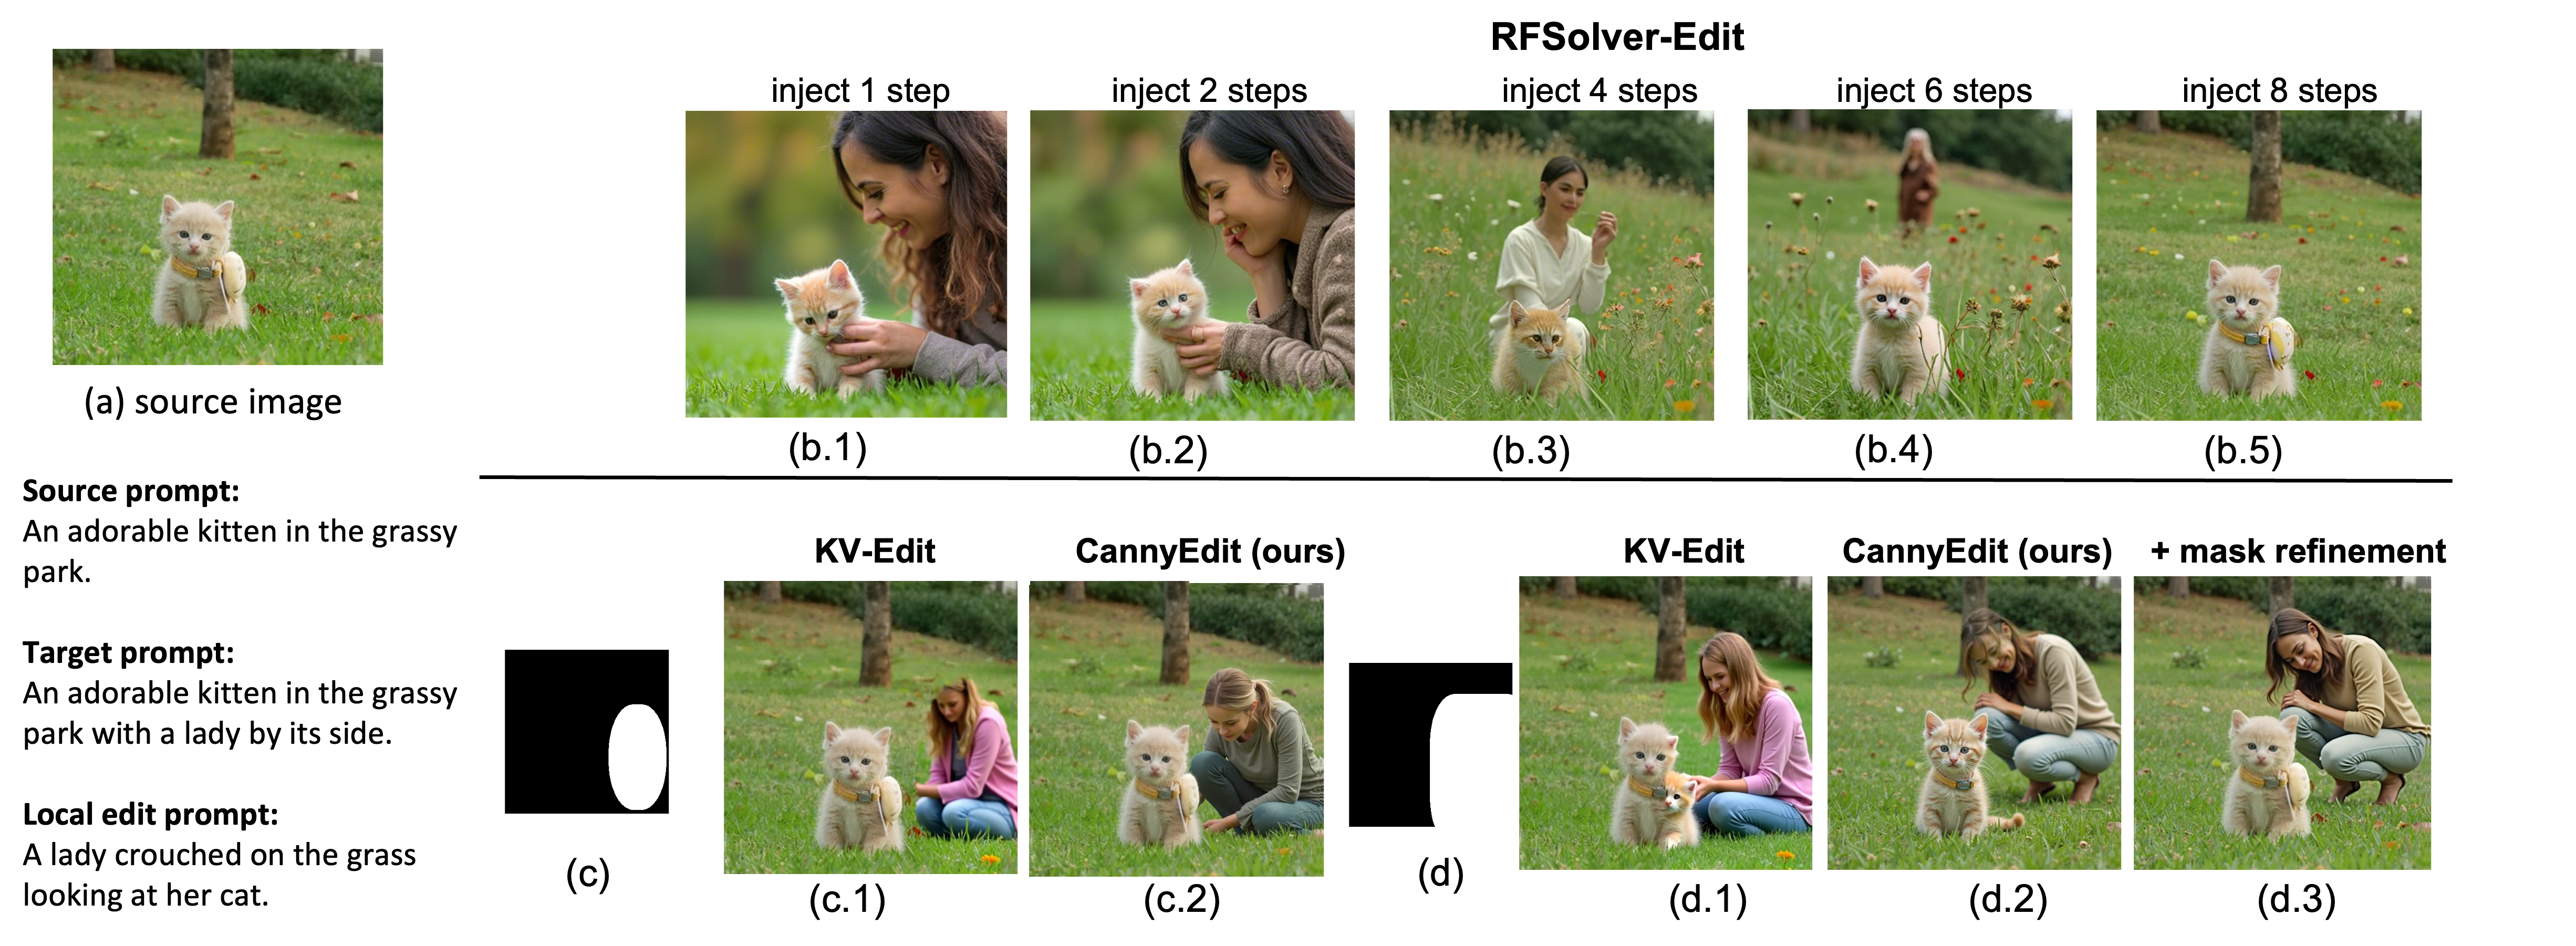
\includegraphics[width=1.\linewidth]{figures/cat.pdf}
      \caption{\textbf{Editing results of different methods.} RFSolver-Edit's outputs fail to balance context fidelity and successful addition simultaneously. While KV-Edit and CannyEdit deliver a better trade-off, CannyEdit results in more natural and seamless edits whereas KV-Edit's results introduce artifacts such as a {partially cropped subject} in (c.1), and {a partially generated extra cat} in (d.1).}
    \label{fig2}
\end{figure}



In summary, we make the following key contributions in this paper:

\vspace{-1mm}
\begin{itemize}[leftmargin=5mm]
\item We propose CannyEdit, a novel image editing method 
% leveraging foundation T2I models and their Canny ControlNet components in a training-free manner. By introducing selective Canny control and soft boundary masking, CannyEdit
that enables high-quality region-based edits that seamlessly blend in with the context. Combined with dual-prompt guidance, CannyEdit produces text-adherent, context-aware results with a strong editability-fidelity balance.
% \textcolor{orange}{Our special treatments on the mask boundary further ensures seamless integration between edited and unedited regions.}

\vspace{-1mm}

\item CannyEdit outperforms strong baselines like KV-Edit~\citep{zhu2025kv}, with up to 10.49\% improvements in real-world image editing tasks. It also surpasses open-source training-based methods such as BrushEdit \citep{li2024brushedit} and PowerPaint \citep{zhuang2023task}. User study shows that CannyEdit produces more natural results with a significantly lower likelihood of being identified as AI-edited than other methods.


\vspace{-1mm}

\item For future research, CannyEdit serves as a flexible and versatile editing framework upon which various image editing solutions can be further developed.
% including insertion, replacement, removal, object transfer, and context modifications, can be further developed.
In principle, our framework can also be easily extended to incorporate other forms of control, such as IP control units \cite{ye2023ip,wang2024instantid}, pose control units \cite{wang2024stablepose,buchheim2025controlling}, etc. CannyEdit also supports multiple edits in one pass of generation.

\end{itemize}

\section{Related work}
\subsection{Training-based image editing methods}

A significant number of studies focus on training-based methods for image editing, which rely on synthetic data generated via large language models and T2I models \citep{brooks2023instructpix2pix, hui2024hq}. While beneficial for teaching models to follow instructions, these methods may not capture all real-world nuances, potentially limiting performance on complex edits. Alternatively, some works collect real-world images and manually annotate data or use task specialists to generate target images \citep{zhang2023magicbrush, wasserman2024paint, wei2024omniedit}. However, scaling these datasets is challenging, and both dataset construction and model training incur considerable computational costs.
The challenge of dataset scalability limits the generalization performance of training-based methods. We argue that training-free methods could be viable alternatives, as they are computationally efficient and preserve the high-quality generation capacity of the foundation T2I model, reducing the risk of overfitting or degradation in image quality.


\vspace{-1mm}

\subsection{Training-free image editing methods}
\vspace{-1mm}





Training-free editing methods typically use a two-stage attention-based pipeline: (1) Inversion: the source image is inverted into the diffusion model's latent space to extract attention features during each denoising step; (2) Source-attention injection: these features are injected into text-image cross-attention during target image generation. Early works like Prompt-to-Prompt \citep{hertz2022prompt} and MasaCtrl \citep{cao2023masactrl} manipulated cross-attention maps in the UNet model between text tokens and image regions. Recent methods \citep{rout2024semantic,wang2024taming,deng2024fireflow,tewel2025addit,zhu2025kv} extend this to more advanced rectified-flow-based transformer models, such as FLUX~\citep{blackforest2024FLUX}. As discussed in Section \ref{Sec:intro}, balancing text adherence in edited regions, preserving unedited context, and achieving seamless integration remain key challenges for existing methods. This work introduces a novel approach that diverges from the attention-based pipeline, without altering the core attention computation process.


\vspace{-1mm}

\subsection{Controllability in T2I generation}
\vspace{-1mm}

Introducing controllability in text-to-image (T2I) generation significantly advances precise image manipulation, unlocking various applications \citep{tan2024ominicontrol,zhang2023adding,li2024controlnet++,li2024unimo,zhao2023uni}. ControlNet \citep{zhang2023adding} is a pivotal framework integrating multiple conditional inputs—such as Canny edge maps for layout, depth maps for spatial arrangement, and skeleton maps for pose control. Specifically, we identify Canny ControlNet as effective for image editing. As an optional plug-and-play module for foundational T2I models, it ensures generated images adhere to both textual prompts and structural details from Canny edges \citep{canny1986computational}. For image editing, we propose to selectively apply the Canny control to enable precise editing in targeted regions while preserving layout consistency elsewhere.


\vspace{-1mm}
\section{Method}

\vspace{-1mm}
\subsection{Preliminaries: FLUX and Canny ControlNet}

\vspace{-1mm}
\begin{wrapfigure}{r}{0.55\textwidth}
  \vspace{-12pt} % Optional: to pull the figure up slightly
    \includegraphics[width=1\linewidth]{figures/FLUX-double-controlnet.pdf}
    \caption{The architecture of multi-stream block in FLUX and in FLUX-ControlNet.}
    \label{fig:FLUX_controlnet}
      \vspace{-6pt} % Optional: reduce space below the figure
\end{wrapfigure}

Our method builds upon FLUX \citep{blackforest2024FLUX}, a prominent open-source T2I foundation model. FLUX uses the Diffusion Transformer (DiT) architecture \citep{peebles2023scalable} and utilizes Rectified Flow (RF) \citep{liu2022flow} to model data-to-noise transformations. It processes multi-modal inputs via a sequence of multi-stream layers (which use separate projection matrices for text and image tokens) and single-stream layers (which use shared projection matrices). The Canny ControlNet \citep{xlabsai2025fluxcontrolnet}, designed for FLUX, integrates duplicates of two multi-stream blocks from FLUX to inject structural layout guidance into it, as shown in Figure \ref{fig:FLUX_controlnet}.


The attention module within the FLUX multi-stream block, shown in Figure \ref{fig:FLUX_controlnet} (a), computes cross-attention between image tokens ($\texttt{I}$) and text tokens ($\texttt{T}$):
% \begin{equation}
% \mathcal{A} = \mathrm{softmax}\left(\frac{[Q_\text{txt}, Q_\texttt{I}] [K_\text{txt}, K_\texttt{I}]^\top}{\sqrt{d_k}}\right),\quad 
% h =  \mathcal{A} \cdot [V_\text{txt}, V_\texttt{I}],\quad 
% h_\texttt{I} = \mathcal{A}_\texttt{I} \cdot [V_\text{txt}, V_\texttt{I}].
% \label{eq:FLUX_attention}
% \end{equation}
% Here, $\mathcal{A}_\texttt{I}$ corresponds to the rows of $\mathcal{A}$ associated with the image tokens. 
\begin{equation}
Z = \begin{bmatrix} Z_\texttt{I}\\Z_\texttt{T}\end{bmatrix} = \mathrm{softmax}\left(\frac{Q K^\top}{\sqrt{d_k}}\right)V,\quad \text{where }
Q = \begin{bmatrix}Q_\texttt{I}\\Q_\texttt{T}\end{bmatrix},\ 
K = \begin{bmatrix}K_\texttt{I}\\K_\texttt{T}\end{bmatrix},\ 
V = \begin{bmatrix}V_\texttt{I}\\V_\texttt{T}\end{bmatrix}.\ 
\label{eq:FLUX_attention}
\end{equation}
%$[Q_\text{txt}, Q_\texttt{I}]$ denotes the concatenated tensor of the text and image queries, obtained by multiplying the text embeddings and image embeddings with their respective query matrices. The term $d_k$ represents the dimension of the key vectors. $\mathcal{A}_\texttt{I}$ corresponds to the rows of $\mathcal{A}$ associated with the image tokens. The same logic applies to the keys and values.
Here, $Q, K, V$ represent the query, key, and value matrices, respectively.

Figure \ref{fig:FLUX_controlnet} (b) illustrates the Canny ControlNet's computational flow (dashed lines). The ControlNet is conditioned on embeddings of Canny edge map tokens and text tokens. Furthermore, the image embedding from the FLUX block is summed with the Canny edge map embedding within the ControlNet. The image token outputs from the FLUX block ($Z_{\texttt{I}}$) and the ControlNet block ($Z^{\prime}_{\texttt{I}}$) are subsequently combined via $Z_{\texttt{I}} \gets Z_{\texttt{I}} + \beta \cdot \mathrm{conv}(Z^{\prime}_{\texttt{I}})$,
where $\mathrm{conv}$ denotes a $1\times1$ convolution layer, and $\beta$ is a hyperparameter controlling the strength of the Canny layout guidance.


\begin{figure}[t]
    \centering
    \includegraphics[width=0.8\linewidth]{figures/framework33.pdf}
    %\vspace{-1mm}
    \caption{\textbf{The inversion-denoising process of CannyEdit.} 1) \emph{inversion}: Starting from the source image, its Canny edge map, and a source prompt \( P_\text{source} \), we use FireFlow~\citep{deng2024fireflow} to obtain the inverted noise \( \mathbf{x}_{t_N} \) and corresponding Canny ControlNet outputs \( \tilde{Z}^{\prime}_{\texttt{I}} \). The immediate noisy latents during the inversion process $\{\mathbf{x}_{t_{1}},...,\mathbf{x}_{t_{N-1}}\}$ are also cached for enhancing the context fidelity. 2) \emph{denoising}: Using the inverted noise \( \mathbf{x}_{t_N} \), we perform guided generation with selective Canny control (via a mask $E$), and dual prompts, \( P_\text{local} \) and \( P_\text{target} \), to provide multi-level text guidance.}
    \label{fig:framework}
    \vspace{-2mm}
\end{figure}



\subsection{Selective Canny control}

Image editing with diffusion models typically employs an inversion-denoising framework. This involves first inverting the source image to obtain an initial latent $\mathbf{x}_{t_N}$ that effectively captures its content at the final timestep, essentially mapping the image back through the diffusion process to its noisy latent representation. We utilize FireFlow \citep{deng2024fireflow} for this inversion step, chosen for its favorable balance between precision and computational cost. A key aspect of our method is that, during this inversion process, while operating on the source image, we apply the Canny ControlNet and cache its outputs ($\tilde{Z}^{\prime}_{\texttt{I}}$) at relevant blocks and timesteps. These cached outputs encode structural guidance derived directly from the source image's Canny edges and features. Optionally, intermediate inverted latents $\mathbf{x}_t$ can also be cached at each timestep.

As illustrated in Figure~\ref{fig:framework}, for the subsequent denoising phase, where the edited image is generated, we leverage these cached outputs via a technique we call \emph{selective Canny control}. Based on a user-provided binary mask $E$ (where $E_{ij}=1$ indicates an editable patch), we apply the cached ControlNet guidance $\tilde{Z}^{\prime}_{\texttt{I}}$ \emph{only} to the masked region ($1-E$). This selective application is mathematically implemented by masking the cached ControlNet output before adding it to the output features:
\begin{equation}
    Z_{\texttt{I}} \gets Z_{\texttt{I}} + \beta\cdot (1-E) \odot \mathrm{conv}(\tilde{Z}^{\prime}_{\texttt{I}}). \label{eq:tweak}
\end{equation}
By applying structural guidance from the source image's Canny edges exclusively to the unedited background region, we effectively preserve its original layout and visual details. Concurrently, the deliberate absence of Canny control within the masked editing region allows the diffusion process there to be guided primarily by the target text prompt, facilitating the desired modifications. Using the pre-computed cached outputs also enhances computational efficiency during the generation phase. 

Further improvements to context preservation and transition smoothness can be achieved through optional cyclical blending with cached latents and attenuating the control strength $\beta$ near the mask boundary. To be specific, when the immediate inverted noisy latents $\{\mathbf{x}_{t_{1}},...,\mathbf{x}_{t_{N-1}}\}$ is cached,  cyclical blending can be applied to the unedited region:  $\mathbf{x}^\text{edit}_{t_\text{blend}}\leftarrow \alpha\cdot\mathbf{x}^\text{edit}_{t_\text{blend}}+(1-\alpha)\cdot\mathbf{x}_{t_\text{blend}}$ where $t_\text{blend}$ is sampled at a pre-defined frequency; The Canny control strength on the mask boundary in the background region is reduced by lowering the $\beta$ value according its distance to the center of the mask (details in Appendix A).



\vspace{-1mm}
\subsection{Dual-prompt guidance}
\label{sec:dualprompt}
\vspace{-1mm}

To achieve text-aligned and seamless edits, we introduce a dual-prompt guidance strategy. This approach combines local prompts, which provide region-specific textual signals, with a global target prompt, which captures interactions between the edited regions and the broader image context. Although termed ``dual-prompt'', this strategy can accommodate multiple local prompts for simultaneous edits in several regions. For simplicity, we describe an implementation with two local prompts guiding two distinct regions; extension to more regions and prompts is straightforward.

\vspace{-1mm}
\subsubsection{General formulation}
\vspace{-1mm}

Let the two image regions be $\texttt{I}_\texttt{1}$ and $\texttt{I}_\texttt{2}$, their corresponding local prompts be $\texttt{T}_\texttt{1}$ and $\texttt{T}_\texttt{2}$, and the global prompt be $\texttt{T}_\texttt{*}$. The number of tokens of these regions/prompts is denoted by $|\cdot|$. At each timestep, the query matrix $Q$ is formed by concatenating the query of these tokens: $ Q= [Q_{\texttt{I}_\texttt{1}}, Q_{\texttt{I}_\texttt{2}}, Q_{\texttt{T}_\texttt{1}}, Q_{\texttt{T}_\texttt{2}}, Q_{\texttt{T}_\texttt{*}}]$. The key $K$ and value $V$ matrices are constructed analogously.

Following prior work \citep{chen2024training}, we implement multi-level and multi-region text guidance in a training-free manner by applying regional text control via an attention mask $M$ within the self-attention module of the FLUX blocks (originally defined in Equation (\ref{eq:FLUX_attention})). The modified attention computation becomes:
\begin{equation}
Z = \mathrm{softmax}\left(\frac{QK^\top}{\sqrt{d_k}} \odot M\right)V, \quad\text{where }M = \begin{bmatrix}
        M_{\texttt{I}\to\texttt{I}} &  M_{\texttt{I}\to\texttt{T}} \\
        M_{\texttt{T}\to\texttt{I}} &  M_{\texttt{T}\to\texttt{T}}
    \end{bmatrix}
\label{eq:masked_attention}
\end{equation}
is the attention mask applied to the concatenated image-text tokens.
% Given the modality correspondence, $ M$ can be denoted as:
% \begin{equation}
    
% \end{equation}
For text-to-text (T2T) attention, $M_{\texttt{T}\to\texttt{T}}$, we prevent information leakage between distinct guidance signals by restricting each text prompt to attend only to its own tokens. This is enforced using a block-diagonal attention mask: $M_{\texttt{T}\to\texttt{T}}=\mathrm{diag}(\mathbf{1}_{|\texttt{T}_\texttt{1}| \times |\texttt{T}_\texttt{1}|}, \mathbf{1}_{|\texttt{T}_\texttt{2}| \times |\texttt{T}_\texttt{2}|},\mathbf{1}_{|\texttt{T}_\texttt{*}| \times|\texttt{T}_\texttt{*}|})$, where $\mathbf{1}_{n \times n}$ is an all-ones matrix of size $n \times n$. This structure enables full self-attention within each prompt while zeroing out off-diagonal blocks to disable cross-prompt interactions.

For text-to-image (T2I) attention, $M_{\texttt{T}\to\texttt{I}}$, local prompts provide guidance to their respective image regions, while the global target prompt interacts with all image regions to capture broader contextual information. This is achieved with:
\begin{equation}
    M_{\texttt{T}\to\texttt{I}} = \begin{bmatrix}
        \mathbf{1}_{|\texttt{T}_\texttt{1}|\times|\texttt{I}_\texttt{1}|} &  \mathbf{0}_{|\texttt{T}_\texttt{1}|\times|\texttt{I}_\texttt{2}|}\\
        \mathbf{0}_{|\texttt{T}_\texttt{2}|\times|\texttt{I}_\texttt{1}|} &  \mathbf{1}_{|\texttt{T}_\texttt{2}|\times|\texttt{I}_\texttt{2}|}\\
         \mathbf{1}_{|\texttt{T}_\texttt{*}|\times|\texttt{I}_\texttt{1}|} &  \mathbf{1}_{|\texttt{T}_\texttt{*}|\times|\texttt{I}_\texttt{2}|}
    \end{bmatrix},
\end{equation}
where $\mathbf{0}_{n \times m}$ denotes an all-zeros matrix. Symmetrically, we let the image-to-text (I2T) attention $M_{\texttt{I}\to\texttt{T}}=(M_{\texttt{T}\to\texttt{I}})^\top$ to allow bidirectional information flow between modalities.
% and symmetrically we let $M_{\texttt{I}\to\texttt{T}}=(M_{\texttt{T}\to\texttt{I}})^\top$, allowing the bidirectional flow of information between the image and text modalities.

Finally, for image-to-image (I2I) attention, $M_{\texttt{I}\to\texttt{I}}$, by default we only allow attention only within each respective region: $M_{\texttt{I}\to\texttt{I}}=\mathrm{diag}(\mathbf{1}_{|\texttt{I}_\texttt{1}| \times |\texttt{I}_\texttt{1}|}, \mathbf{1}_{|\texttt{I}_\texttt{2}| \times |\texttt{I}_\texttt{2}|})$, thereby maintaining the integrity of region-specific processing.

\subsubsection{Adjustments for practical editing tasks}

The default block-diagonal $M_{\texttt{I}\to\texttt{I}}$ is suitable when all regions are considered independently editable. However, for practical editing tasks, this mask can be adjusted based on the roles of different regions. For instance, when adding new content, let $\texttt{I}_\texttt{1}$ be the edit region and $\texttt{I}_\texttt{2}$ be the background region. The local prompt $\texttt{T}_\texttt{2}$ for the background region can be the source image's original prompt. In this scenario, $M_{\texttt{I}\to\texttt{I}}$ can be modified to:
\begin{equation}
    M_{\texttt{I}\to\texttt{I}}(\texttt{I}_\texttt{1}\to\texttt{I}_\texttt{2})%(\texttt{I}_\texttt{1}, \texttt{I}_\texttt{2})
    % = \mathrm{diag}(\mathbf{1}_{|\texttt{I}_\texttt{1}|^2}, \mathbf{1}_{|\texttt{I}_\texttt{2}|^2})+ \begin{bmatrix}
    %     \mathbf{0}_{|\texttt{I}_\texttt{1}|\times|\texttt{I}_\texttt{1}|} &  \mathbf{0}_{|\texttt{I}_\texttt{1}|\times|\texttt{I}_\texttt{2}|}\\
    %     \mathbf{1}_{|\texttt{I}_\texttt{2}|\times|\texttt{I}_\texttt{1}|} &  \mathbf{0}_{|\texttt{I}_\texttt{2}|\times|\texttt{I}_\texttt{2}|}
    % \end{bmatrix}
    =
    \begin{bmatrix}
        \mathbf{1}_{|\texttt{I}_\texttt{1}|\times|\texttt{I}_\texttt{1}|} &  \mathbf{1}_{|\texttt{I}_\texttt{1}|\times|\texttt{I}_\texttt{2}|}\\
        \mathbf{0}_{|\texttt{I}_\texttt{2}|\times|\texttt{I}_\texttt{1}|} &  \mathbf{1}_{|\texttt{I}_\texttt{2}|\times|\texttt{I}_\texttt{2}|}
    \end{bmatrix}.
    \label{eq:i2i_1}
\end{equation}
This adjustment, through the $\mathbf{1}_{|\texttt{I}_\texttt{1}|\times|\texttt{I}_\texttt{2}|}$ block, allows the edit region $\texttt{I}_\texttt{1}$ to attend to the background region $\texttt{I}_\texttt{2}$. This enables the model to integrate contextual information from the background, leading to a more context-aware edit. This masking approach can be extended to scenarios with multiple editable regions while preserving background integrity.


To further enhance seamless blending between edited and background regions, we refine I2I attention involving the background area adjacent to the edit boundary. Let $\texttt{I}_\texttt{1}$ be the edit region, $\texttt{I}_\texttt{:}$ be the portion of the background region at the boundary of $\texttt{I}_\texttt{1}$, and $\texttt{I}_\texttt{2}$ be the remaining background region (distinct from $\texttt{I}_\texttt{:}$ and $\texttt{I}_\texttt{1}$). The I2I attention mask is then defined as
\begin{equation}
M_{\texttt{I}\to\texttt{I}}(\texttt{I}_\texttt{1}\to\texttt{I}_\texttt{2};\  \texttt{I}_\texttt{1}\leftrightarrow\texttt{I}_\texttt{:}\!\leftrightarrow \texttt{I}_\texttt{2}) =   \begin{bmatrix}
        \mathbf{1}_{|\texttt{I}_\texttt{1}|\times|\texttt{I}_\texttt{1}|} &  \mathbf{1}_{|\texttt{I}_\texttt{1}|\times|\texttt{I}_\texttt{:}|}&\mathbf{1}_{|\texttt{I}_\texttt{1}|\times|\texttt{I}_\texttt{2}|}\\

\boxed{\mathbf{1}_{|\texttt{I}_\texttt{:}|\times|\texttt{I}_\texttt{1}|}} &  \mathbf{1}_{|\texttt{I}_\texttt{:}|\times|\texttt{I}_\texttt{:}|}&\mathbf{1}_{|\texttt{I}_\texttt{:}|\times|\texttt{I}_\texttt{2}|}\\
\mathbf{0}_{|\texttt{I}_\texttt{2}|\times|\texttt{I}_\texttt{1}|} &  \mathbf{1}_{|\texttt{I}_\texttt{2}|\times|\texttt{I}_\texttt{:}|}&\mathbf{1}_{|\texttt{I}_\texttt{2}|\times|\texttt{I}_\texttt{2}|}\\
    \end{bmatrix}.
\label{eq:i2i_2}
\end{equation}
The key change from Equation (\ref{eq:i2i_1}) is the introduction of the boxed block $\mathbf{1}_{|\texttt{I}_\texttt{:}|\times|\texttt{I}_\texttt{1}|}$, which allows the background region at the boundary ($\texttt{I}_\texttt{:}$) to attend to the edit region ($\texttt{I}_\texttt{1}$), enabling the model to incorporate contextual cues from the edited content into these boundary areas. Consequently, the boundary regions can better align visually and semantically with the edits, reducing artifacts and improving overall image coherence.


\subsubsection{Prompting strategies for various editing tasks}



The specifics of local prompts vary depending on the editing task. For object insertion and replacement, local prompts describe the objects to be introduced or the new objects that will substitute existing ones. For object removal, the default local prompt that we use is ``empty background''. We also employ classifier-free guidance \citep{ho2022classifier} by using descriptions of the objects targeted for removal as negative local prompts. A more detailed discussion on applying these techniques to diverse editing tasks—such as object transfer while preserving object shapes, or modifying the environment/atmosphere of a specific region—is provided in {Appendix B}, where we also explore how our method can be extended to handle multiple edits within a single generation pass.






\vspace{-1mm}
\section{Experiment}
\label{Sec:experiment}

\vspace{-1mm}

\textbf{Baselines.} We mainly compare CannyEdit with open-source methods: (1) Training-based approaches including BrushEdit~\cite{li2024brushedit} based on UNet diffusion models, FLUX Fill~\cite{blackforest2024FLUX} and PowerPaint-FLUX~\cite{zhuang2023task} based on FLUX~\cite{blackforest2024FLUX}. Note that the original PowerPaint in \cite{blackforest2024FLUX} is based on UNet diffusion model, for a fairer comparison, we trained a new version based on FLUX with the provided training dataset. (2) Training-free approaches including P2P~\cite{hertz2022prompt}, MasaCtrl~\cite{cao2023masactrl} based on DDIM \citep{song2022denoisingdiffusionimplicitmodels}, and RF-Inversion~\cite{rout2024semantic}, RFSolver-Edit~\cite{wang2024taming}, KV-Edit~\cite{zhu2025kv} based on Rectified
Flow. %In summary, there are eight prevalent image inpainting and editing methods for evaluation. 

\textbf{Datasets.} We introduce the \textbf{R}eal \textbf{I}mage \textbf{C}omplex \textbf{E}diting Benchmark ({RICE-Bench}) to address the lack of realistic interactions among objects in existing real-world image editing benchmarks~\citep{sheynin2024emu,gu2024multi}. RICE-Bench consists of 80 images capturing real, complex editing scenarios for object insertion, replacement, and removal. It is designed to better evaluate \textit{context fidelity}, \textit{text adherence}, and \textit{editing seamlessness} in real-world editing tasks. Example images from the benchmark are shown in {Figures \ref{logo}, \ref{fig2}}, with more examples and details of data curation provided in Appendix D. In short, we curated the data from open datasets \citep{wasserman2024paint,ju2024pnp} and our own private data.
We also conduct evaluations on PIE-Bench~\cite{ju2024pnp}, a dataset of 620 real-world and synthetic images spanning 9 diverse editing tasks.
Following \cite{li2024brushedit, xu2023infedit, zhu2025kv}, we exclude the style transfer task to focus on region-based image editing.


\textbf{Implementation details.} We implement our method based on FLUX.1-[dev]~\cite{blackforest2024FLUX} and FLUX-Canny-ControlNet~\cite{xlabsai2025fluxcontrolnet}, using 50 denoising steps and a guidance value of 4.0. The strength parameter of Canny control $\beta$ is set to 0.8 in the inversion and for the non-mask-boundary background region. We apply cyclical blending with $\alpha=0.5$ every 5 steps. Other methods were implemented based on their official code releases' default settings unless otherwise specified. More details, including machines used, hyperparameters, and a computational cost analysis for CannyEdit, are provided in {Appendix C}.


\textbf{Metrics.}  For RICE-Bench, we evaluate edits using three metrics: \textbf{Context Fidelity (CF)}, \textbf{Text Adherence (TA)}, and \textbf{Trade-off Score (TO Score)}. CF measures cosine similarity between original and edited images using DINO embeddings~\citep{caron2021emerging}. TA assesses adherence to text prompts via GroundingDINO~\citep{liu2024grounding} top-1 bounding-box prediction confidence $p_{\text{gdino}}(\textit{image}, \textit{edited object})$ for the edited object, defined as the confidence difference between edited and source images: positive in $p_{\text{gdino}}(\textit{edited}, \textit{edited object})-p_{\text{gdino}}(\textit{source}, \textit{edited object})$ for addition/replacement edits and reversed in $p_{\text{gdino}}(\textit{source}, \textit{removed object})-p_{\text{gdino}}(\textit{edited}, \textit{removed object})$ for removal edits to measure the successful elimination of the object. TO Score balances fidelity and editability, computed as $\text{TO Score} = \text{CF} + \text{TA}$. RICE-Bench also includes a user study evaluating editing seamlessness by gauging users' ability to identify AI-generated edits. For PIE-Bench, following \citet{zhu2025kv}, we use seven metrics: HPSv2~\citep{wu2023human} and aesthetic scores~\citep{schuhmann2022laionb} (image quality), PSNR~\citep{huynh2008scope}, LPIPS~\citep{zhang2018perceptual}, and MSE (background preservation), and CLIP score~\citep{radford2021learning} and Image Reward~\citep{xu2023imagereward} (text adherence).




\vspace{-2mm}
\subsection{Experiment results on RICE-Bench}

\vspace{-1mm}


\begin{table*}[t]
\begin{center} 
\footnotesize
\setlength{\tabcolsep}{1.70mm} %
\caption{Results of automatically computed metrics comparing with representative methods on RICE-Bench. The ``inject'' for RFSolver-Edit denotes the number of denoising steps where the source image's attention features are injected. The metrics are context fidelity (CF), Text Adherence (TA), and Trade-off Score (TO Score), which measures the trade-off for editability and fidelity. \textbf{Bold} and \underline{underlined} values represent the best and second-best TO scores respectively.}

\resizebox{0.95\textwidth}{!}{
\begin{tabular}{lcccccccccc}
\toprule
 & \multicolumn{3}{c}{Add} & \multicolumn{3}{c}{Removal} &\multicolumn{3}{c}{Replace} & Avg.\\
\cmidrule(lr){2-4} \cmidrule(lr){5-7} \cmidrule(lr){8-10} \cmidrule(lr){11-11}
Metrics & $\textup{CF}_{\times 10^2}^{\uparrow}$ & $\textup{TA}_{\times 10^2}^{\uparrow}$ & TO Score& $\textup{CF}_{\times 10^2}^{\uparrow}$ & $\textup{TA}_{\times 10^2}^{\uparrow}$ & TO Score& $\textup{CF}_{\times 10^2}^{\uparrow}$ & $\textup{TA}_{\times 10^2}^{\uparrow}$ & TO Score& TO Score\\
\midrule
RFSolver-Edit ($\textup{inject}=2$)~\cite{wang2024taming} & 71.77 & 22.65 & 94.42 & 42.99 & 39.05 & 82.04 & 47.44 & 9.22 & 56.66 & 77.71\\
RFSolver-Edit ($\textup{inject}=8$)~\cite{wang2024taming} & 99.13 & 2.14 & 101.27 & 79.34 & 2.94 & 82.28 & 67.89 & 5.03 & 72.92 & 85.49\\
KV-Edit~\cite{zhu2025kv} & 93.91 & 17.25 & \underline{111.16} & 69.81 & 16.62 & 86.43 & 64.72 & 12.36 & \underline{77.08} & \underline{91.56}\\
BrushEdit~\cite{li2024brushedit} & 87.26 & 18.98 & 106.24 & 63.43 & 31.29 & \underline{94.72} & 59.11 & 7.40 & 66.51 & 89.16\\
FLUX Fill~\cite{blackforest2024FLUX} & 88.21 & 21.62 & 109.83 & 70.94 & 10.91 & 81.85 & 60.20 & 8.13 & 68.33 & 86.67\\
PowerPaint-FLUX~\cite{zhuang2023task} & 84.63 & 24.34 & 108.97 & 62.31 & 21.40 & 83.71 & 60.75 & 8.92 & 69.67 & 87.45\\
\midrule
\textbf{CannyEdit (Ours)} & 88.72 & 28.12 & \textbf{116.84} & 63.28 & 34.22 & \textbf{97.50} & 64.43 & 16.77 & \textbf{81.20} & \textbf{98.51}\\
\bottomrule
\end{tabular}}
\label{tab:rice-comparison}
\end{center}

\begin{center} 
\footnotesize
\setlength{\tabcolsep}{1.85mm} %
\caption{Results of user study comparing CannyEdit with representative methods on RICE-Bench ({\scriptsize $\pm${}} denotes 95\% confidence interval). In Task1, participants identify AI-edited images from paired real (\emph{Real}) and generated (\emph{Gen}) images. Seamless edits yield selection ratios close to random chance (50\%), as achieved by CannyEdit. In Task2, users directly compare CannyEdit against other methods; lower selection ratios for ``ours'' indicate superior editing seamlessness of CannyEdit.}

\

\resizebox{1.\textwidth}{!}{
\begin{tabular}{lcccccccc}
\toprule
 & \multicolumn{4}{c}{General User (96 participants)} & \multicolumn{4}{c}{Expert (41 participants)} \\
 \cmidrule(lr){2-5}\cmidrule(lr){6-9}
%\midrule
& \multicolumn{2}{c}{{Generated vs. Real}} & \multicolumn{2}{c}{CannyEdit vs. Others} &\multicolumn{2}{c}{Generated vs. Real} & \multicolumn{2}{c}{CannyEdit vs. Others}\\
%\midrule
 \cmidrule(lr){2-3} \cmidrule(lr){4-5}\cmidrule(lr){6-7}\cmidrule(lr){8-9}
 Ratio regarded as AIGC (\%) & $\textup{Gen}^{\downarrow}$ & $\textup{Real}^{\uparrow}$ & $\textup{Ours}^{\downarrow}$ & $\textup{Itself}^{\downarrow}$ & $\textup{Gen}^{\downarrow}$ & $\textup{Real}^{\uparrow}$ & $\textup{Ours}^{\downarrow}$ & $\textup{Itself}^{\downarrow}$\\
\midrule
%Random choices & 50.00  & 50.00 & 50.00 & 50.00 & 50.00 & 50.00 & 50.00 & 50.00\\
%\midrule
KV-Edit~\cite{zhu2025kv} & 86.96{\scriptsize $\pm${7.19}}  & 13.04{\scriptsize $\pm${7.19}} & \textbf{37.50}{\scriptsize $\pm${5.72}} & 62.50{\scriptsize $\pm${5.72}} & 89.09{\scriptsize $\pm${9.24}} & 10.91{\scriptsize $\pm${9.24}} & \textbf{37.69}{\scriptsize $\pm${10.2}} & 62.31{\scriptsize $\pm${10.2}}\\
BrushEdit~\cite{li2024brushedit} & 79.20{\scriptsize $\pm${8.99}} & 20.80{\scriptsize $\pm${8.99}} & \textbf{30.00}{\scriptsize $\pm${4.90}} & 70.00{\scriptsize $\pm${4.90}} & \underline{82.00}{\scriptsize $\pm${12.1}} & \underline{18.00}{\scriptsize $\pm${12.1}} & \textbf{19.29}{\scriptsize $\pm${9.99}} & 80.71{\scriptsize $\pm${9.99}}\\
PowerPaint-FLUX~\cite{zhuang2023task} & \underline{76.08}{\scriptsize $\pm${5.49}} & \underline{23.92}{\scriptsize $\pm${5.49}} & \textbf{38.08}{\scriptsize $\pm${6.66}} & 61.92{\scriptsize $\pm${6.66}} & 88.00{\scriptsize $\pm${6.57}} & 12.00{\scriptsize $\pm${6.57}} & \textbf{33.85}{\scriptsize $\pm${7.32}} & 66.15{\scriptsize $\pm${7.32}}\\
\midrule
\textbf{CannyEdit (Ours)} & \textbf{49.20}{\scriptsize $\pm${3.56}} & \textbf{50.80}{\scriptsize $\pm${3.56}} & N/A & N/A & \textbf{42.00}{\scriptsize $\pm${8.12}} & \textbf{58.00}{\scriptsize $\pm${8.12}} & N/A & N/A\\
\bottomrule
\end{tabular}}
\label{tab:rice-human-study} 
\end{center}
\vspace{-2mm}
\end{table*}



In Table~\ref{tab:rice-comparison}, our method demonstrates superior performance in automatic evaluations compared to existing techniques. Achieving the highest TO score across three editing tasks, it strikes the best balance between image editability and fidelity. In contrast, methods like RFSolver-Edit face a notable trade-off, either adhering closely to the text instruction while negatively impacting the image context with fewer steps, or preserving context but failing to fully implement the desired edits with more steps. KV-Edit similarly prioritizes context preservation but at the expense of significantly reduced text adherence. Training-based methods also struggle to achieve a comparable equilibrium.

To complement the automatic metrics and systematically assess the perceived seamlessness of the edits, we conducted a user study with a total of 137 participants, comprising 96 general users with limited AIGC experience and 41 experts with formal training or experience.
The study involved two tasks where participants viewed pairs of images and were asked to identify which image was most likely AI-edited. In Task 1, an image edited by our method was compared against a real, unedited image. In Task 2, an image generated by our method is compared against one from another method. To minimize bias, the presentation order of images and questions was randomized. Only successful edits with high text adherence scores were included. A preliminary screening test filtered out participants with low accuracy in distinguishing AI-edited from real images, ensuring data reliability. More details of the user study are provided in Appendix E.

The results, presented in Table~\ref{tab:rice-human-study}, highlight our method's ability to produce highly seamless edits. In Task 1, general users identified images from our method as AI-edited only 49.20\% of the time, while experts did so even less frequently at 42.00\%. This indicates that our edited images were often indistinguishable from real ones. Conversely, images from alternative methods were much more readily identified as AI-generated, with detection rates ranging from 76.08\% to 89.09\%. Consistent with Task 1, in Task 2, images generated by our method were consistently less likely to be perceived as AI-edited when compared directly to outputs from other methods, further underscoring the superior seamlessness of our editing approach.


\vspace{-1mm}
\subsection{Experiment results on PIE-Bench}
\vspace{-1mm}
\begin{figure}[h!]
\vspace{-1mm}
\begin{tabular}{@{\hskip 1pt} p{\dimexpr\textwidth/9\relax}
                   @{\hskip 1pt} p{\dimexpr\textwidth/9\relax}
                   @{\hskip 1pt} p{\dimexpr\textwidth/9\relax}
                   @{\hskip 1pt} p{\dimexpr\textwidth/9\relax}
                   @{\hskip 10pt} p{\dimexpr\textwidth/9\relax}
                   @{\hskip 1pt} p{\dimexpr\textwidth/9\relax}
                   @{\hskip 1pt} p{\dimexpr\textwidth/9\relax}
                   @{\hskip 1pt} p{\dimexpr\textwidth/9\relax} @{}}

\multicolumn{4}{c}{\scriptsize \textbf{Add} a hat to the table with flowers.} & 
\multicolumn{4}{c}{\scriptsize \textbf{Add} a deer in the forest. }  \\
\includegraphics[width=\linewidth,  height=1.5cm]{figures/f3/1_1.jpg} &
\includegraphics[width=\linewidth,  height=1.5cm]{figures/f3/1_2.png} &
\includegraphics[width=\linewidth,  height=1.5cm]{figures/f3/1_3.jpg} &
\includegraphics[width=\linewidth,  height=1.5cm]{figures/f3/1_4.jpg} &
\includegraphics[width=\linewidth,  height=1.5cm]{figures/f3/2_1.jpg} &
\includegraphics[width=\linewidth,  height=1.5cm]{figures/f3/2_2.png} &
\includegraphics[width=\linewidth,  height=1.5cm]{figures/f3/2_3.jpg} &
\includegraphics[width=\linewidth,  height=1.5cm]{figures/f3/2_4.jpg} \\[-1pt]


\multicolumn{1}{c}{{\scriptsize Input}} &\multicolumn{1}{c}{{\scriptsize Mask}} &\multicolumn{1}{c}{{\scriptsize CannyEdit}}&\multicolumn{1}{c}{{\scriptsize KV-Edit}} &\multicolumn{1}{c}{{\scriptsize Input}} &\multicolumn{1}{c}{{\scriptsize Mask}} &\multicolumn{1}{c}{{\scriptsize CannyEdit}}&\multicolumn{1}{c}{{\scriptsize KV-Edit}}\\
\multicolumn{2}{c}{\scriptsize $\text{LPIPS}({\times 10^3})\downarrow $} &\multicolumn{1}{c}{{\scriptsize 51.84}} & \multicolumn{1}{c}{{\scriptsize \textbf{22.90}}} &\multicolumn{2}{c}{\scriptsize $\text{LPIPS}({\times 10^3})\downarrow $} &\multicolumn{1}{c}{{\scriptsize 35.52}}&\multicolumn{1}{c}{{\scriptsize\bf 16.44}}\\
\multicolumn{2}{c}{\scriptsize $\text{PSNR}\uparrow$}&\multicolumn{1}{c}{{\scriptsize 22.85}} & \multicolumn{1}{c}{{\scriptsize \textbf{26.54}}} &\multicolumn{2}{c}{\scriptsize $\text{PSNR}\uparrow$}&\multicolumn{1}{c}{{\scriptsize 26.61}}&\multicolumn{1}{c}{{\scriptsize\bf 27.90}}\\
\end{tabular}
\caption{Visual examples of our CannyEdit and KV-Edit \cite{zhu2025kv} on PIE examples along with their quantitative results on background preservation.}
\label{fig:pie_example}
\end{figure}




{We extend our evaluation to PIE-Bench which involves more images in various editing tasks. The result is displayed in Table~\ref{tab:pie-comparison}. As for text alignment, CannyEdit significantly outperforms other methods both in CLIP similarity($22.44\rightarrow \textbf{25.36}$) and Image Reward($5.71\rightarrow \textbf{8.20}$). Our method also keeps a competitive level in image quality.} The accuracy of masked region preservation achieved by CannyEdit is numerically inferior to that of KV-Edit. However, as illustrated by the examples in Figure \ref{fig:pie_example}, the background preservation metrics tend to penalize the more natural and complete results generated by CannyEdit, which may not effectively reflect the quality of the background preservation.





\begin{table*}[t]

\begin{center} 
\footnotesize
\setlength{\tabcolsep}{1.85mm} %
\caption{{Comparison with other methods on PIE-Bench.} VAE$^*$ denotes the inherent reconstruction error through VAE reconstruction only. Except the result of ours, other results follow \cite{zhu2025kv}.}
\resizebox{0.76\textwidth}{!}{
\begin{tabular}{lccccccc}
\toprule
\multirow{3}{*}[0.8ex]{Metrics} & \multicolumn{2}{c}{Image Quality} & \multicolumn{3}{c}{Background Preservation} &\multicolumn{2}{c}{Text Adherence} \\
\cmidrule(lr){2-3}\cmidrule(lr){4-6}\cmidrule(lr){7-8}   &  $\textup{HPS}_{\times 10^2}^{\uparrow}$ & $\textup{AS}^{\uparrow}$ & $\textup{PSNR}^\uparrow$ & $\textup{LPIPS}_{\times 10^3}^{\downarrow}$ & $\textup{MSE}_{\times 10^4}^{\downarrow}$ & $\textup{CLIP Sim}^{\uparrow}$ & $\textup{IR}_{\times10}^{\uparrow}$\\
\midrule
VAE$^*$ & 24.93 & 6.37 & 37.65 & 7.93 & 3.86 & 19.69 & -3.65\\
\midrule
P2P~\cite{hertz2022prompt} & 25.40 & 6.27& 17.86 & 208.43 & 219.22 & 22.24 & 0.017 \\
MasaCtrl~\cite{cao2023masactrl} & 23.46 & 5.91 & 22.20 & 105.74 & 86.15 & 20.83 & -1.66\\
RF-Inversion~\cite{rout2024semantic} & \textbf{27.99} & \textbf{6.74} & 20.20 & 179.73 & 139.85 & 21.71 & 4.34\\
RFSolver-Edit~\cite{wang2024taming} & \underline{27.60} & \underline{6.56}& 24.44& 113.20& 56.26& 22.08& 5.18\\
KV-Edit~\cite{zhu2025kv} & 27.21 & 6.49 & \textbf{35.87}& \textbf{9.92}& \textbf{4.69}& 22.39 & 5.63\\
BrushEdit~\cite{li2024brushedit} & 25.81 & 6.17 & 32.16 & \underline{17.22} & \underline{8.46} & \underline{22.44} & 3.33\\
FLUX Fill~\cite{blackforest2024FLUX} & 25.76 & 6.31 & \underline{32.53} & 25.59 & 8.55 & 22.40 & \underline{5.71}\\
%Powerpaint-FLUX~\cite{zhuang2023task} & & & & & & & \\
\midrule
\textbf{CannyEdit (Ours)} & 27.19 & 6.38 & 32.18 & 26.38 & 9.79& \textbf{25.36} & \textbf{8.20}\\
\bottomrule
\end{tabular}}
\label{tab:pie-comparison} 
\end{center}

\begin{center} 
\footnotesize
\setlength{\tabcolsep}{1.05mm} %
\caption{{Ablation study for CannyEdit on adding and replacement examples of RICE-Bench.} The evaluation metrics follow these in Table \ref{tab:rice-comparison}. \emph{CC} denotes Canny Control, \emph{DP} is for Dual-Prompt Guidance and  \emph{CB} means cyclical blending. For comparison, we also copy the results of KV-Edit here.}

\

\resizebox{0.76\textwidth}{!}{
\begin{tabular}{llcccccc}
\toprule
&  & \multicolumn{3}{c}{Add} & \multicolumn{3}{c}{Replace}\\
\cmidrule(lr){3-5}\cmidrule(lr){6-8}
 & & $\textup{CF}_{\times 10^2}^{\uparrow}$ & $\textup{TA}_{\times 10^2}^{\uparrow}$ & $\textup{TO Score}^{\uparrow}$ & $\textup{CF}_{\times 10^2}^{\uparrow}$ & $\textup{TA}_{\times 10^2}^{\uparrow}$ & $\textup{TO Score}^{\uparrow}$ \\
\midrule
% Baseline & w/o CC, w/o Rx & 81.4/22.0 & 103.4 & ---- & ---- & 48.7/14.9 & 63.6 \\
KV-Edit (baseline) && 93.91 & 17.25 & 111.16 &64.72&12.36&77.08 \\ %\midrule
\textbf{CannyEdit (Ours)} &  &{88.72} &{28.12} & \textbf{116.84} & {64.43}&{16.77} & \textbf{81.20} \\
\midrule
\multirow{3}{*}{\begin{tabular}[c]{@{}c@{}}Variants \\ \arraybackslash of \emph{CC}\end{tabular}} & 
selective \emph{CC} from current T2I   &84.81 &27.93 &112.74 &55.24&13.89  & 69.13   \\
&w/o \emph{CC} & 79.73&{26.29} & 106.02 & 51.51&11.83 & 63.34 \\
 & full \emph{CC}  & {93.41}&19.73 & {113.14} & {64.02}&12.51 & {76.53} \\
\midrule
\multirow{2}{*}{\begin{tabular}[c]{@{}c@{}}Variants \\ \arraybackslash of \emph{DP}\end{tabular}} & local prompt only  & {93.43}&10.23 & 103.66 & 58.92&{17.09} & 76.01 \\
 & target prompt only& 85.04&24.96 & 109.00& 60.82&15.43 & 76.25 \\
\midrule 
Variant of \emph{CB} &blend at every step & 93.24&22.09&115.33 &65.12&13.08 & 78.20\\
\bottomrule
\end{tabular}}
\label{tab:ablation-study} 
\end{center}
\vspace{-2mm}
\end{table*}

% \begin{figure}[htbp]
%     \centering
%     % First image pair
%     \begin{subfigure}[b]{0.2\textwidth}
%         \includegraphics[width=\linewidth]{figures/tm/image1.png}
%         \caption*{(a.1)}
%     \end{subfigure}
%     \begin{subfigure}[b]{0.2\textwidth}
%         \includegraphics[width=\linewidth]{figures/tm/image2.png}
%         \caption*{(a.2)}
%     \end{subfigure}
%     % Second image pair
%     \begin{subfigure}[b]{0.2\textwidth}
%         \includegraphics[width=\linewidth]{figures/tm/3941.jpeg}
%         \caption*{(b.1)}
%     \end{subfigure}
%     \begin{subfigure}[b]{0.2\textwidth}
%         \includegraphics[width=\linewidth]{figures/tm/image5.jpeg}
%         \caption*{(b.2)}
%     \end{subfigure}
%     \caption{Visual examples highlight the importance of special treatments at the boundary between edited and unedited regions. Without treatments, (a.1) and (b.1) show rough transitions, while (a.2) and (b.2) demonstrate smoother results with treatments of reduced canny control and attention adjustment applied.}
%     \label{fig:treaments}
% \end{figure}

\vspace{-1mm}
\subsection{Ablation study}

\vspace{-1mm}

We evaluate key modules of CannyEdit using addition and replacement examples from RICE-Bench (Table~\ref{tab:ablation-study}). Avoiding cached ControlNet outputs, by either using selective Canny ControlNet's outputs for current T2I denoising process or completely omitting Canny control (1st and 2nd variant of \emph{CC}), significantly reduces context fidelity. Conversely, using full Canny control improves context preservation but weakens adherence to textual instructions (still outperforms KV-Edit). Ablations on dual-prompt guidance confirm that both local and global prompts are crucial for effective edits.

CannyEdit introduces cyclic blending, periodically integrating background features from the original image. While blending at every denoising step better preserves context, it reduces precision in following text instructions (yet remains superior to KV-Edit). Additionally, specialized boundary treatments, such as reduced Canny control and modification of attention masks on the mask boundary region, are essential for smooth visual transitions. Without these treatments, noticeable artifacts and unnatural boundaries can appear (see Appendix F.5 for examples). Our evaluations use oval-shaped masks for additions by default, but Appendix F.6 demonstrates that CannyEdit is robust to other mask shapes, including rectangular and user-drawn styles.



\vspace{-1mm}
\subsection{Qualitative examples}

\vspace{-1mm}
Visual examples in Figures \ref{logo} and \ref{fig2} demonstrate that CannyEdit achieves a strong balance between context fidelity, text adherence, and editing seamlessness. More examples comparing CannyEdit with different open-source methods are in Appendix F.1. Examples of applying CannyEdit to other editing tasks and more comparison results with close-source models, GPT-4o \citep{OpenAI2025Introducing4O} and Gemini 2.0 Flash \citep{google_gemini2025} are provided in Appendix F.2 and F.3. Our method can also support multiple edits at one pass of generation, an example is given in Figure \ref{logo} (a), more multi-edit examples are given in Appendix F.4.  

%  \begin{figure}[h!]
% \vspace{-5mm}
% \begin{center}
% \begin{tabular}{@{\hskip 1.2pt} p{\dimexpr\textwidth/9\relax}
%                    @{\hskip 5pt} p{\dimexpr\textwidth/9\relax}
%                    @{\hskip 1.2pt} p{\dimexpr\textwidth/9\relax}
%                    @{\hskip 1.2pt} p{\dimexpr\textwidth/9\relax}
%                    @{\hskip 5pt} p{\dimexpr\textwidth/9\relax}
%                    @{\hskip 1.2pt} p{\dimexpr\textwidth/9\relax}
%                    @{\hskip 1.2pt} p{\dimexpr\textwidth/9\relax} @{}}

%  & \multicolumn{3}{c}{\tiny (a) \textbf{Add} a woman embracing the man.} & 
% \multicolumn{3}{c}{\tiny (b) \textbf{Replace} the man with a woman}  \\
% \includegraphics[width=0.8\linewidth,  height=1.2cm]{figures/f2/1_1.png} &
% \includegraphics[width=0.8\linewidth,  height=1.2cm]{figures/f2/1_2.png} &
% \includegraphics[width=0.8\linewidth,  height=1.2cm]{figures/f2/1_3.jpg} &
% \includegraphics[width=0.8\linewidth,  height=1.2cm]{figures/f2/1_4.jpg} &
% \includegraphics[width=0.8\linewidth,  height=1.2cm]{figures/f2/1_5.jpg} &
% \includegraphics[width=0.8\linewidth,  height=1.2cm]{figures/f2/1_6.png} &
% \includegraphics[width=0.8\linewidth,  height=1.2cm]{figures/f2/1_7.jpg} \\[-1pt]

%  & \multicolumn{3}{c}{\tiny (c) \textbf{Replace} the dog with a boy.} & 
% \multicolumn{3}{c}{\tiny (d) \textbf{Remove} the boy.} \\
% \includegraphics[width=0.8\linewidth,  height=1.2cm]{figures/f2/2_1.jpg} &
% \includegraphics[width=0.8\linewidth,  height=1.2cm]{figures/f2/2_2.png} &
% \includegraphics[width=0.8\linewidth,  height=1.2cm]{figures/f2/2_3.png} &
% \includegraphics[width=0.8\linewidth,  height=1.2cm]{figures/f2/2_4.png} &
% \includegraphics[width=0.8\linewidth,  height=1.2cm]{figures/f2/2_5.png} &
% \includegraphics[width=0.8\linewidth,  height=1.2cm]{figures/f2/2_6.jpg} &
%  \includegraphics[width=0.8\linewidth,  height=1.2cm]{figures/f2/2_7.png}  \\[-1pt]

%  & \multicolumn{3}{c}{\tiny (e) \textbf{Replace} the male player with a female player.} &
% \multicolumn{3}{c}{\tiny (f) \textbf{Remove} the football player.} \\
% \includegraphics[width=0.8\linewidth,  height=1.2cm]{figures/f2/3_1.jpg} &
% \includegraphics[width=0.8\linewidth,  height=1.2cm]{figures/f2/3_2.png} &
% \includegraphics[width=0.8\linewidth,  height=1.2cm]{figures/f2/3_3.png} &
% \includegraphics[width=0.8\linewidth,  height=1.2cm]{figures/f2/3_4.png} &
% \includegraphics[width=0.8\linewidth,  height=1.2cm]{figures/f2/3_5.png} &
% \includegraphics[width=0.8\linewidth,  height=1.2cm]{figures/f2/3_6.png} &
% \includegraphics[width=0.8\linewidth,  height=1.2cm]{figures/f2/3_7.png}  \\
% \multicolumn{1}{c}{{\scriptsize Input}} &\multicolumn{1}{l}{{\tiny  CannyEdit}} &\multicolumn{1}{l}{{\tiny  KV-Edit}}&\multicolumn{1}{l}{{\tiny PowerPaint}} &\multicolumn{1}{l}{{\tiny  CannyEdit}} &\multicolumn{1}{l}{{\tiny  KV-Edit}} &\multicolumn{1}{l}{{\tiny PowerPaint}}  \\
% \end{tabular}
% \caption{Visual examples of our CannyEdit, KV-Edit~\citep{zhu2025kv}, and PowerPaint-FLUX~\cite{zhuang2023task}. The samples are from the RICE-Bench (detailed text prompts and masks are omitted here; see Appendix F.1). \kc{[Maybe move this to the appendix to save space]}}
% \label{fig:qualitative_RICE22}
% \end{center}
% \vspace{-5mm}
% \end{figure}


% \textcolor{red}{In Figure \ref{fig:qualitative_RICE}, we displays qualitative examples of regional image editing across Add, Replace and Removal. The samples are taken from the manipulated RICE-Bench.}





\vspace{-1mm}
\section{Conclusion}
\vspace{-1mm}

This paper introduces CannyEdit, a novel training-free method for region-based image editing. By utilizing the plug-and-play Canny ControlNet module, we apply the selective Canny control guidance to the foundational T2I model, enabling precise editability in the target region while preserving layout consistency and contextual integrity in other areas. Combined with dual-prompt text guidance, which incorporates both local and global textual information, our method achieves a strong balance between text adherence, contextual fidelity, and seamless editing. We hope that CannyEdit inspires further exploration and innovation in applying Canny layout control into various generation tasks, providing more flexible and accessible tools for creative and practical applications.  Additionally, we discuss the limitations of our method and potential avenues for improvement in Appendix G.


\newpage
\bibliography{main}
\bibliographystyle{plainnat}




%%%%%%%%%%%%%%%%%%%%%%%%%%%%%%%%%%%%%%%%%%%%%%%%%%%%%%%%%%%%

% \appendix

% \section{Technical Appendices and Supplementary Material}
% Technical appendices with additional results, figures, graphs and proofs may be submitted with the paper submission before the full submission deadline (see above), or as a separate PDF in the ZIP file below before the supplementary material deadline. There is no page limit for the technical appendices.

%%%%%%%%%%%%%%%%%%%%%%%%%%%%%%%%%%%%%%%%%%%%%%%%%%%%%%%%%%%%

\newpage
\section*{NeurIPS Paper Checklist}

\begin{enumerate}

\item {\bf Claims}
    \item[] Question: Do the main claims made in the abstract and introduction accurately reflect the paper's contributions and scope?
    \item[] Answer: \answerYes{} % Replace by \answerYes{}, \answerNo{}, or \answerNA{}.
    \item[] Justification: We pinpoint the area we are in and list contributions clearly. Please refer to Abstract and Introduction \ref{Sec:intro}.
    \item[] Guidelines:
    \begin{itemize}
        \item The answer NA means that the abstract and introduction do not include the claims made in the paper.
        \item The abstract and/or introduction should clearly state the claims made, including the contributions made in the paper and important assumptions and limitations. A No or NA answer to this question will not be perceived well by the reviewers. 
        \item The claims made should match theoretical and experimental results, and reflect how much the results can be expected to generalize to other settings. 
        \item It is fine to include aspirational goals as motivation as long as it is clear that these goals are not attained by the paper. 
    \end{itemize}

\item {\bf Limitations}
    \item[] Question: Does the paper discuss the limitations of the work performed by the authors?
    \item[] Answer: \answerYes{} % Replace by \answerYes{}, \answerNo{}, or \answerNA{}.
    \item[] Justification: We discussed the limitations in Appendix G.
    \item[] Guidelines:
    \begin{itemize}
        \item The answer NA means that the paper has no limitation while the answer No means that the paper has limitations, but those are not discussed in the paper. 
        \item The authors are encouraged to create a separate "Limitations" section in their paper.
        \item The paper should point out any strong assumptions and how robust the results are to violations of these assumptions (e.g., independence assumptions, noiseless settings, model well-specification, asymptotic approximations only holding locally). The authors should reflect on how these assumptions might be violated in practice and what the implications would be.
        \item The authors should reflect on the scope of the claims made, e.g., if the approach was only tested on a few datasets or with a few runs. In general, empirical results often depend on implicit assumptions, which should be articulated.
        \item The authors should reflect on the factors that influence the performance of the approach. For example, a facial recognition algorithm may perform poorly when image resolution is low or images are taken in low lighting. Or a speech-to-text system might not be used reliably to provide closed captions for online lectures because it fails to handle technical jargon.
        \item The authors should discuss the computational efficiency of the proposed algorithms and how they scale with dataset size.
        \item If applicable, the authors should discuss possible limitations of their approach to address problems of privacy and fairness.
        \item While the authors might fear that complete honesty about limitations might be used by reviewers as grounds for rejection, a worse outcome might be that reviewers discover limitations that aren't acknowledged in the paper. The authors should use their best judgment and recognize that individual actions in favor of transparency play an important role in developing norms that preserve the integrity of the community. Reviewers will be specifically instructed to not penalize honesty concerning limitations.
    \end{itemize}

\item {\bf Theory assumptions and proofs}
    \item[] Question: For each theoretical result, does the paper provide the full set of assumptions and a complete (and correct) proof?
    \item[] Answer: \answerNA{} % Replace by \answerYes{}, \answerNo{}, or \answerNA{}.
    \item[] Justification: We do not have theoretical results.
    \item[] Guidelines:
    \begin{itemize}
        \item The answer NA means that the paper does not include theoretical results. 
        \item All the theorems, formulas, and proofs in the paper should be numbered and cross-referenced.
        \item All assumptions should be clearly stated or referenced in the statement of any theorems.
        \item The proofs can either appear in the main paper or the supplemental material, but if they appear in the supplemental material, the authors are encouraged to provide a short proof sketch to provide intuition. 
        \item Inversely, any informal proof provided in the core of the paper should be complemented by formal proofs provided in appendix or supplemental material.
        \item Theorems and Lemmas that the proof relies upon should be properly referenced. 
    \end{itemize}

    \item {\bf Experimental result reproducibility}
    \item[] Question: Does the paper fully disclose all the information needed to reproduce the main experimental results of the paper to the extent that it affects the main claims and/or conclusions of the paper (regardless of whether the code and data are provided or not)?
    \item[] Answer: \answerYes{} % Replace by \answerYes{}, \answerNo{}, or \answerNA{}.
    \item[] Justification: We elucidated datasets used, baselines to compare, and implementation details of our method in Section \ref{Sec:experiment} and Appendix C.
    \item[] Guidelines:
    \begin{itemize}
        \item The answer NA means that the paper does not include experiments.
        \item If the paper includes experiments, a No answer to this question will not be perceived well by the reviewers: Making the paper reproducible is important, regardless of whether the code and data are provided or not.
        \item If the contribution is a dataset and/or model, the authors should describe the steps taken to make their results reproducible or verifiable. 
        \item Depending on the contribution, reproducibility can be accomplished in various ways. For example, if the contribution is a novel architecture, describing the architecture fully might suffice, or if the contribution is a specific model and empirical evaluation, it may be necessary to either make it possible for others to replicate the model with the same dataset, or provide access to the model. In general. releasing code and data is often one good way to accomplish this, but reproducibility can also be provided via detailed instructions for how to replicate the results, access to a hosted model (e.g., in the case of a large language model), releasing of a model checkpoint, or other means that are appropriate to the research performed.
        \item While NeurIPS does not require releasing code, the conference does require all submissions to provide some reasonable avenue for reproducibility, which may depend on the nature of the contribution. For example
        \begin{enumerate}
            \item If the contribution is primarily a new algorithm, the paper should make it clear how to reproduce that algorithm.
            \item If the contribution is primarily a new model architecture, the paper should describe the architecture clearly and fully.
            \item If the contribution is a new model (e.g., a large language model), then there should either be a way to access this model for reproducing the results or a way to reproduce the model (e.g., with an open-source dataset or instructions for how to construct the dataset).
            \item We recognize that reproducibility may be tricky in some cases, in which case authors are welcome to describe the particular way they provide for reproducibility. In the case of closed-source models, it may be that access to the model is limited in some way (e.g., to registered users), but it should be possible for other researchers to have some path to reproducing or verifying the results.
        \end{enumerate}
    \end{itemize}


\item {\bf Open access to data and code}
    \item[] Question: Does the paper provide open access to the data and code, with sufficient instructions to faithfully reproduce the main experimental results, as described in supplemental material?
    \item[] Answer: \answerNo{} % Replace by \answerYes{}, \answerNo{}, or \answerNA{}.
    \item[] Justification: The code and dataset will be released to public upon the acceptance of the paper.
    \item[] Guidelines:
    \begin{itemize}
        \item The answer NA means that paper does not include experiments requiring code.
        \item Please see the NeurIPS code and data submission guidelines (\url{https://nips.cc/public/guides/CodeSubmissionPolicy}) for more details.
        \item While we encourage the release of code and data, we understand that this might not be possible, so “No” is an acceptable answer. Papers cannot be rejected simply for not including code, unless this is central to the contribution (e.g., for a new open-source benchmark).
        \item The instructions should contain the exact command and environment needed to run to reproduce the results. See the NeurIPS code and data submission guidelines (\url{https://nips.cc/public/guides/CodeSubmissionPolicy}) for more details.
        \item The authors should provide instructions on data access and preparation, including how to access the raw data, preprocessed data, intermediate data, and generated data, etc.
        \item The authors should provide scripts to reproduce all experimental results for the new proposed method and baselines. If only a subset of experiments are reproducible, they should state which ones are omitted from the script and why.
        \item At submission time, to preserve anonymity, the authors should release anonymized versions (if applicable).
        \item Providing as much information as possible in supplemental material (appended to the paper) is recommended, but including URLs to data and code is permitted.
    \end{itemize}


\item {\bf Experimental setting/details}
    \item[] Question: Does the paper specify all the training and test details (e.g., data splits, hyperparameters, how they were chosen, type of optimizer, etc.) necessary to understand the results?
    \item[] Answer: \answerYes{} % Replace by \answerYes{}, \answerNo{}, or \answerNA{}.
    \item[] Justification: We elaborated the implementation details of our method in Section \ref{Sec:experiment} and in Appendix C.
    \item[] Guidelines:
    \begin{itemize}
        \item The answer NA means that the paper does not include experiments.
        \item The experimental setting should be presented in the core of the paper to a level of detail that is necessary to appreciate the results and make sense of them.
        \item The full details can be provided either with the code, in appendix, or as supplemental material.
    \end{itemize}

\item {\bf Experiment statistical significance}
    \item[] Question: Does the paper report error bars suitably and correctly defined or other appropriate information about the statistical significance of the experiments?
    \item[] Answer: \answerYes{} % Replace by \answerYes{}, \answerNo{}, or \answerNA{}.
    \item[] Justification: We conducted well-designed user study to evaluate the seamlessness of editing methods. The statistical confidence is also reported in Table~\ref{tab:rice-human-study}.
    \item[] Guidelines:
    \begin{itemize}
        \item The answer NA means that the paper does not include experiments.
        \item The authors should answer "Yes" if the results are accompanied by error bars, confidence intervals, or statistical significance tests, at least for the experiments that support the main claims of the paper.
        \item The factors of variability that the error bars are capturing should be clearly stated (for example, train/test split, initialization, random drawing of some parameter, or overall run with given experimental conditions).
        \item The method for calculating the error bars should be explained (closed form formula, call to a library function, bootstrap, etc.)
        \item The assumptions made should be given (e.g., Normally distributed errors).
        \item It should be clear whether the error bar is the standard deviation or the standard error of the mean.
        \item It is OK to report 1-sigma error bars, but one should state it. The authors should preferably report a 2-sigma error bar than state that they have a 96\% CI, if the hypothesis of Normality of errors is not verified.
        \item For asymmetric distributions, the authors should be careful not to show in tables or figures symmetric error bars that would yield results that are out of range (e.g. negative error rates).
        \item If error bars are reported in tables or plots, The authors should explain in the text how they were calculated and reference the corresponding figures or tables in the text.
    \end{itemize}

\item {\bf Experiments compute resources}
    \item[] Question: For each experiment, does the paper provide sufficient information on the computer resources (type of compute workers, memory, time of execution) needed to reproduce the experiments?
    \item[] Answer: \answerYes{} % Replace by \answerYes{}, \answerNo{}, or \answerNA{}.
    \item[] Justification:The usage of computing resources and the analysis of computational cost for our CannyEdit are provided in Appendix C.
    \item[] Guidelines:
    \begin{itemize}
        \item The answer NA means that the paper does not include experiments.
        \item The paper should indicate the type of compute workers CPU or GPU, internal cluster, or cloud provider, including relevant memory and storage.
        \item The paper should provide the amount of compute required for each of the individual experimental runs as well as estimate the total compute. 
        \item The paper should disclose whether the full research project required more compute than the experiments reported in the paper (e.g., preliminary or failed experiments that didn't make it into the paper). 
    \end{itemize}
    
\item {\bf Code of ethics}
    \item[] Question: Does the research conducted in the paper conform, in every respect, with the NeurIPS Code of Ethics \url{https://neurips.cc/public/EthicsGuidelines}?
    \item[] Answer: \answerYes{} % Replace by \answerYes{}, \answerNo{}, or \answerNA{}.
    \item[] Justification: We reviewed and followed the NeurIPS Code of Ethics.
    \item[] Guidelines:
    \begin{itemize}
        \item The answer NA means that the authors have not reviewed the NeurIPS Code of Ethics.
        \item If the authors answer No, they should explain the special circumstances that require a deviation from the Code of Ethics.
        \item The authors should make sure to preserve anonymity (e.g., if there is a special consideration due to laws or regulations in their jurisdiction).
    \end{itemize}


\item {\bf Broader impacts}
    \item[] Question: Does the paper discuss both potential positive societal impacts and negative societal impacts of the work performed?
    \item[] Answer: \answerYes{} % Replace by \answerYes{}, \answerNo{}, or \answerNA{}.
    \item[] Justification: We discussed the societal impact of our method in Appendix G.
    \item[] Guidelines:
    \begin{itemize}
        \item The answer NA means that there is no societal impact of the work performed.
        \item If the authors answer NA or No, they should explain why their work has no societal impact or why the paper does not address societal impact.
        \item Examples of negative societal impacts include potential malicious or unintended uses (e.g., disinformation, generating fake profiles, surveillance), fairness considerations (e.g., deployment of technologies that could make decisions that unfairly impact specific groups), privacy considerations, and security considerations.
        \item The conference expects that many papers will be foundational research and not tied to particular applications, let alone deployments. However, if there is a direct path to any negative applications, the authors should point it out. For example, it is legitimate to point out that an improvement in the quality of generative models could be used to generate deepfakes for disinformation. On the other hand, it is not needed to point out that a generic algorithm for optimizing neural networks could enable people to train models that generate Deepfakes faster.
        \item The authors should consider possible harms that could arise when the technology is being used as intended and functioning correctly, harms that could arise when the technology is being used as intended but gives incorrect results, and harms following from (intentional or unintentional) misuse of the technology.
        \item If there are negative societal impacts, the authors could also discuss possible mitigation strategies (e.g., gated release of models, providing defenses in addition to attacks, mechanisms for monitoring misuse, mechanisms to monitor how a system learns from feedback over time, improving the efficiency and accessibility of ML).
    \end{itemize}
    
\item {\bf Safeguards}
    \item[] Question: Does the paper describe safeguards that have been put in place for responsible release of data or models that have a high risk for misuse (e.g., pretrained language models, image generators, or scraped datasets)?
    \item[] Answer: \answerNo{} % Replace by \answerYes{}, \answerNo{}, or \answerNA{}.
    \item[] Justification: We will provide related safeguards for the code and dataset which will be released to public upon the acceptance of the paper.
    \item[] Guidelines:
    \begin{itemize}
        \item The answer NA means that the paper poses no such risks.
        \item Released models that have a high risk for misuse or dual-use should be released with necessary safeguards to allow for controlled use of the model, for example by requiring that users adhere to usage guidelines or restrictions to access the model or implementing safety filters. 
        \item Datasets that have been scraped from the Internet could pose safety risks. The authors should describe how they avoided releasing unsafe images.
        \item We recognize that providing effective safeguards is challenging, and many papers do not require this, but we encourage authors to take this into account and make a best faith effort.
    \end{itemize}

\item {\bf Licenses for existing assets}
    \item[] Question: Are the creators or original owners of assets (e.g., code, data, models), used in the paper, properly credited and are the license and terms of use explicitly mentioned and properly respected?
    \item[] Answer: \answerYes{} % Replace by \answerYes{}, \answerNo{}, or \answerNA{}.
    \item[] Justification: We cited related papers and code we refer to in this paper. And we also followed corresponding requirements of license.
    \item[] Guidelines:
    \begin{itemize}
        \item The answer NA means that the paper does not use existing assets.
        \item The authors should cite the original paper that produced the code package or dataset.
        \item The authors should state which version of the asset is used and, if possible, include a URL.
        \item The name of the license (e.g., CC-BY 4.0) should be included for each asset.
        \item For scraped data from a particular source (e.g., website), the copyright and terms of service of that source should be provided.
        \item If assets are released, the license, copyright information, and terms of use in the package should be provided. For popular datasets, \url{paperswithcode.com/datasets} has curated licenses for some datasets. Their licensing guide can help determine the license of a dataset.
        \item For existing datasets that are re-packaged, both the original license and the license of the derived asset (if it has changed) should be provided.
        \item If this information is not available online, the authors are encouraged to reach out to the asset's creators.
    \end{itemize}

\item {\bf New assets}
    \item[] Question: Are new assets introduced in the paper well documented and is the documentation provided alongside the assets?
    \item[] Answer: \answerYes{} % Replace by \answerYes{}, \answerNo{}, or \answerNA{}.
    \item[] Justification: We introduced details of our newly proposed benchmark in Section \ref{Sec:experiment}.
    \item[] Guidelines:
    \begin{itemize}
        \item The answer NA means that the paper does not release new assets.
        \item Researchers should communicate the details of the dataset/code/model as part of their submissions via structured templates. This includes details about training, license, limitations, etc. 
        \item The paper should discuss whether and how consent was obtained from people whose asset is used.
        \item At submission time, remember to anonymize your assets (if applicable). You can either create an anonymized URL or include an anonymized zip file.
    \end{itemize}

\item {\bf Crowdsourcing and research with human subjects}
    \item[] Question: For crowdsourcing experiments and research with human subjects, does the paper include the full text of instructions given to participants and screenshots, if applicable, as well as details about compensation (if any)? 
    \item[] Answer: \answerYes{} % Replace by \answerYes{}, \answerNo{}, or \answerNA{}.
    \item[] Justification: We introduced tasks to finish by participants with details in Section \ref{Sec:experiment}. And the examples of tasks were listed in Appendix E.
    \item[] Guidelines:
    \begin{itemize}
        \item The answer NA means that the paper does not involve crowdsourcing nor research with human subjects.
        \item Including this information in the supplemental material is fine, but if the main contribution of the paper involves human subjects, then as much detail as possible should be included in the main paper. 
        \item According to the NeurIPS Code of Ethics, workers involved in data collection, curation, or other labor should be paid at least the minimum wage in the country of the data collector. 
    \end{itemize}

\item {\bf Institutional review board (IRB) approvals or equivalent for research with human subjects}
    \item[] Question: Does the paper describe potential risks incurred by study participants, whether such risks were disclosed to the subjects, and whether Institutional Review Board (IRB) approvals (or an equivalent approval/review based on the requirements of your country or institution) were obtained?
    \item[] Answer: \answerNA{} % Replace by \answerYes{}, \answerNo{}, or \answerNA{}.
    \item[] Justification: No risks that could harm human physical and mental health were found in our experimental design.
    \item[] Guidelines:
    \begin{itemize}
        \item The answer NA means that the paper does not involve crowdsourcing nor research with human subjects.
        \item Depending on the country in which research is conducted, IRB approval (or equivalent) may be required for any human subjects research. If you obtained IRB approval, you should clearly state this in the paper. 
        \item We recognize that the procedures for this may vary significantly between institutions and locations, and we expect authors to adhere to the NeurIPS Code of Ethics and the guidelines for their institution. 
        \item For initial submissions, do not include any information that would break anonymity (if applicable), such as the institution conducting the review.
    \end{itemize}

\item {\bf Declaration of LLM usage}
    \item[] Question: Does the paper describe the usage of LLMs if it is an important, original, or non-standard component of the core methods in this research? Note that if the LLM is used only for writing, editing, or formatting purposes and does not impact the core methodology, scientific rigorousness, or originality of the research, declaration is not required.
    %this research? 
    \item[] Answer: \answerNA{} % Replace by \answerYes{}, \answerNo{}, or \answerNA{}.
    \item[] Justification: LLMs are not the core in our method.
    \item[] Guidelines:
    \begin{itemize}
        \item The answer NA means that the core method development in this research does not involve LLMs as any important, original, or non-standard components.
        \item Please refer to our LLM policy (\url{https://neurips.cc/Conferences/2025/LLM}) for what should or should not be described.
    \end{itemize}

\end{enumerate}


\end{document}